\chapter{Project Background}
\label{chap:antecedentes}


This chapter resumes the main subjects acquired during the accomplishment of the GEO-Cloud project.  The novel architecture proposed in this project for EO processing carries the absence of this kind of platforms to compare with. In this way, the study of the state of the art will be done focalising in some aspects of cloud computing platforms, federated testbeds, networking, satellite systems, and so on. As consequence, this section depicts the different thematic areas .
The conceptual map showed in Figure~\ref{fig:intr-conceptual-map} presents the sections and subsections of this chapter. Thereby in Earth Observation Satellites area, the different concepts for creating and modelling a satellite for earth imaging, its data management and orbital definitions is studied. In high-level languages, some scripting languages are compared. In Networking section, different network impairments and several tools for acquiring these are depicted. In Federated Infrastructre section, the testbeds that Fed4FIRE platform is composed by are explained.

\begin{figure}[!h]
\begin{center}
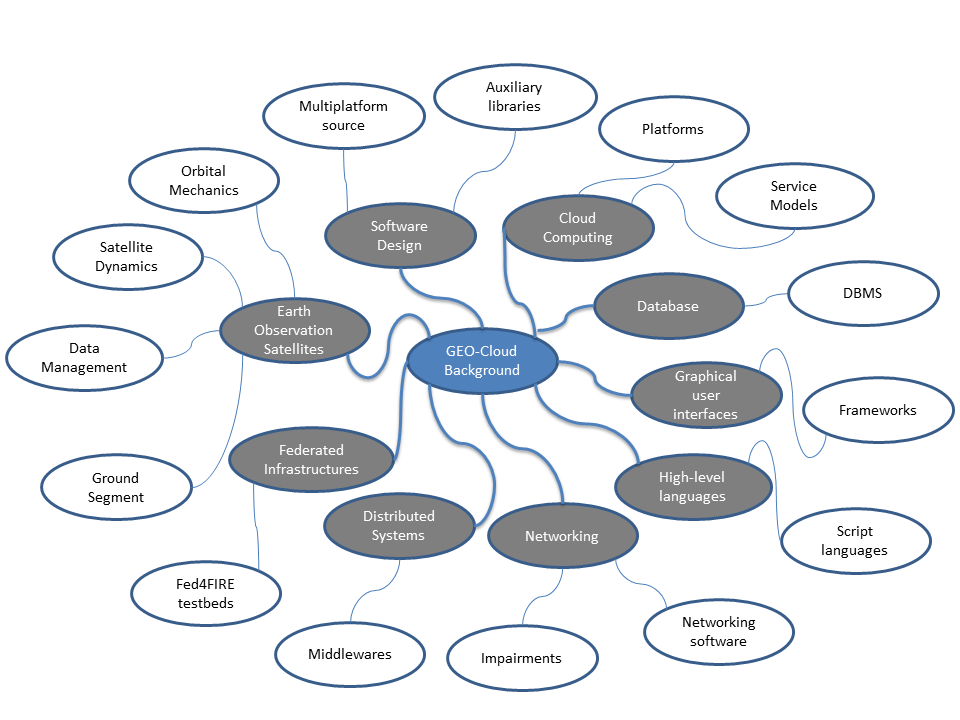
\includegraphics[width=1\textwidth]{statement/background-geocloud.png}
\caption{Conceptual Map of this chapter.}
\label{fig:intr-conceptual-map}
\end{center}
\end{figure}

In the section that explains the Graphical User Interfaces background, several
frameworks for developing GUIs are depicted. In Database section, differents
database management systems are compared. The distributed systems section
explains and compares some middlewares as Hadoop or ZeroC Ice for developing
distributed applications.
Finally, in the Software Design section discusses the requirements for building multiplatform code, and other ancillary libraries required by the detailed objectives of GEO-Cloud.

\section{Earth Observation Satellites}

In this section, different areas of aeronautics are involved. Orbital
Mechanics which defines and calculates the satellite orbits for rounding around
the world;  Spatial Telescopes which contributes with the payload parameters as
\ac{GSD} and Swath among others; finally, the data management which mission consist of processing on fly, storing
and sending the science and ancillary data from satellite to Ground Segment.

\subsection{Orbital Mechanics}

This science~\cite{http://en.wikipedia.org/wiki/Orbital_mechanics} studies the motion of the satellite considered as a point with no
mass in space which is affected by \emph{Newton's Laws of Motion}and \emph{Newton's Law of
Universal Gravitation}.
\emph{The Newton's Law of Universal Gravitation} says that \emph{any two bodies in the
universe attract each other with a force that is directly proportional to the
product of their masses and inversely proportional to the square of the distance
between them.}
%~\cite{http://en.wikipedia.org/wiki/Newton\%27s_law_of_universal_gravitation}

\begin{equation}
F = G* {\frac {m_1*m_2}{r^2}}
\end{equation}
where $F$ is the force between the masses, $G$ is the gravitational constant
($6.67x10^{-11}$), $m_1$ and $m_2$ are the first and second mass respectively
and $r$ is the distance between the centers of the masses.

Orbital Mechanics focuses on the trajectories of the
spacecrafts, maneuvers for orbital acquisition, orbit maintenance, end of life
disposal, etcetera.

Spacecrafts motion  is governed by the \emph{Kepler's Laws of Planetary Motion}
%~\cite{http://en.wikipedia.org/wiki/Kepler\%27s_laws_of_planetary_motion}
which can be derived from \emph{Newton's Laws}. These laws are the following:
\begin{enumerate}
\item The orbit of a planet is an ellipse with the Sun at one of the two foci.
\item A line segment joining a planet and the Sun sweeps out equal areas during
  equal intervals of time.
\item The square of the orbital period of a planet is proportional to the cube
  of the semi-major axis of its orbit.
\end{enumerate}


\subsection{Spatial Telescopes }

The \ac{EO} satellites carry on board telescopes pointing to the Earth in order
to acquire images of the surface. The information can be obtained in several
kinds of spectral bands as visible, near infra-red, thermal, etcetera. This
mission employes visible multispectral telescopes distributed in a constellation of satellites
to obtain daily a global map. For selecting the telescopes, the Swath and \ac{GSD}
have been analised. The number of satellites is dependent on the width of the
swath and the telescope resolution is required to achive quality
images for the mission.

Depending on the spectral bands employed for imaging, the applications are
different. Scientific applications as soil categorization, vegetation analisys,
oceanography use hyperspectral imagers which offers information about hundreds
of bands. 

Other applications as traffic monitoring, urban development,
surveillance commonly require multispectral imagers with visible bands.

\subsection{Data Management}

Each satellite of the constellation acquires images which have five spectral
bands into the visible spectrum. When this spectral data is
obtained by telescopes, it is necesary to convert from analogical to digital
data. This proces is carried out using 12 bits per pixel for codifying the
intensity signal level with a digital value. Then, the digital data is stored and pre-processed on
board. 

During the pre-processing activity, some meta-data that is well known as ancillary
data, is added. The ancillary data enriches the acquired sector of image by adding
some geolocated information and transmission auxiliary meta-data for communication
protocols. \\All the above pre-processed data is agregated in the
internal storage for downloading when the satellite comes into a visibility zone
of a ground station. At the moment the satellite enters in a footprint of a
ground station, the acquired images at real time and the stored images are
downloaded into ground station. \\Sending data is made multiplexing the
communication channel within two ways. The first part of the total bandwidth
is used for downloading the acquired images at real time and the other part of
the rest of bandwidth performs the download of the stored images into the
internal storages.

\subsection{Ground Segment}

The Ground Segment is composed by the antennas, the control center and the
infrastructures for processing and distributing images named processing
data center. 

The current industries of \ac{EO} imaging perform the processing, distributing, and
selling on premises. The steps are the following:
\begin{enumerate}
\item First, the antenas recieves all the data from satellites and store it.
\item Once the data is into the antenna, the processing data center obtains the
  images from the ground stations.
\item The data center starts to process available images.
\item When a image has been processed is sent for archiving and
  cataloguing. 
\item Finally, the image is available for end-users.
\end{enumerate}

The arquitecture on-cloud proposed in this project, reduces the delivery
end-user time making shorter the cataloguing and archiving times.

The control center manages the satellites, schedule mission plannings and
collects telemetry but not interferes in downloading nor processing images.


\section{High-level languages}

For the development of the project, \ac{XML}, \ac{JSON},\emph{Python} and \emph{Bash} languages has
been used. The first, \ac{XML}, has been used for building the configuration file of
the Orchestrator component and to obtain the selected nodes by \emph{JFed}
application. Then \ac{JSON} has been used to create the experiment descriptor for
\bonfire platform. The rest of them are scripting languages. The source of the
components of the cloud has been developed using \emph{Python} and the interconnections
between modules and others secundary funcionalities, in \emph{Bash script}.

\subsection{XML}
\ac{XML} is a markup language that defines a set of rules for encoding
documents in a format that is both human-readable and machine-readable. Most of
actual software use it for configuring or for updating its configuration on fly.

\subsection{JSON}

\ac{JSON} is a lightweight language for data interchage between applications. The
simplicity of \ac{JSON} results very simple and human-readable way to transmit data
objects consisting of attribute-value pairs. Web applications are using this
language substituting \ac{XML} because parsing and generating \ac{JSON} is more efficient
and quick. The \bonfire interface uses it for creating experiment descriptors
ought to the resources provided by the platform can be translated into objects
and its features.

\subsection{Scripting languages}

The Scripting technics consist of use a interpreted programming language in
order to provide advanced mechanisms for specifying funcionalities of an
application. The most important features of a scripting language are that is not
compiled and it permits effortless development. Also, some interpreted languages
are multiplatform because is not necessary to compile the source for running in
target platform. 


\subsubsection{Python}
https://www.python.org/
\emph{Python} is a object oriented language, although permits imperative and functional
programming. It does not need to compile the source because it is
interpreted. It permits a flexible development because it is dynamic type and in
this project, the most important feature why this language has been used,
consist of it is multiplatform. With this feature, the software is able to be
executed in any platform. The current version is 2.7.4 and it offers several
useful and multipourpose libraries as \emph{matlib, pthread, mysqllib, pdb} and so on.

\subsubsection{Bash Script}

Really, \emph{Bash} is not a language, is a command language interpreter for the \ac{GNU}
operative system. \emph{Bash} is fully compatible with other command language
interpreters like \emph{sh} or \emph{ksh}, so the source developed by \emph{Bash}, normally, is
portable. 
However, the \emph{Bash} language is also known as \emph{Bash}. The Bash scripts contains
commands for being executed by the interpreter. This way provides a direct line
to communicate with the operative system and to make some funcionalities ad-hoc.
The \emph{Bash} language consists of several sentences that the operative system is
able to read and translate in order to play a specific action. All the currents
\emph{Linux} distributions contains a Bash interpret. 

\subsubsection{Ruby}
https://www.ruby-lang.org/en/
\emph{Ruby} is a object-oriented, cross-platform, general-purpose and dynamic
programming language. It was designed and developed by \emph{Yukihiro
  Matsumoto}. This language has a dynamic type influenced by Groovy, Falcon and
other ones. It permits a easy, flexible and agile development. 


\subsubsection{Lua}
http://www.lua.org/
\emph{Lua} is a lightweight,cross-platform, prototype-based, object-oriented programming
language. It was designed and developed by \emph{Roberto Lerusalimschy}. This
language is influenced by C++, Modula and Scheme among others. It provides
native data structures as tables, records and associative arrays which this
structure perform hight throughput.


\section{Networking}

For simulating an environment as real as possible in GEO-Cloud, the impairments  of the networks between both Ground Stations and Cloud Platform
and between both Cloud Platform and end-users had to be acquired. Also, features
like bandwidth is obtained in order to stablish the maximum throughput of
channel over \vw.

There are several simulators that
calculates the value of these network feautures roughly but the obtained results
may be wrong o not accurating. Therefore, a subexperiment explained in
Section~\ref{sec:planetlab} for acquiring these values is implemented. 

\subsection{Impairments}

The communication though the Internet is not perfect because there are many
sources or random events that affect traffic packets that are traversing a
network differently at any given moment. This is a main
subject to take into account when a network is being modelling. The main
impairments
%~\cite{http://iwl.com/white-papers/network-impairments/causes-and-correlation}
 of a network are the following:

\begin{itemize}
\item \emph{Packet Loss:} This is simply the disappearance of a packet that was
  transmitted or ought to have been transmitted.
\item \emph{Packet Delay:} Also known as ``Latency'' is the amount of time that elapses between the time a
  packet is transmited to physical environment until the packet is received by
  target. This delay is composed by three types of delay times: Propagation
  delay which is the time that the packet waste arriving destination;
  Routing/Switching delay that is the time that the routers or
  switches waste in processing the packet; finally the Queuing delays that is
  the time that the packet is queued in any intermediate hardware of the entire network.
\item \emph{Jitter:} Jitter is a measure of the variation in the packet delay
  experienced by a numer of packets. 
\item \emph{Packet Duplication:} May occurs when one packet become two or more
  identical packets.
\item \emph{Packet Corruption:} It occurs when the payload of the packet (even a bit)
  is damaged but the packet continues to flow towards the destination instead of
  being discarded.
\end{itemize}

For GEO-Cloud project, the impairments to be acquired are \emph{Packet Loss} and
\emph{Packet Delay} that permit modelling a simulated and close to realily network.


\subsection{Networking Software}

In the networking subject, there are lots of tools that permit to obtain the
features values for the metrics defined above in a network. 
For measuring the throughput, bandwidth and loss-rate the following tools are interesting:

\begin{itemize}
\item \emph{Microsoft's NTttcp~{http://gallery.technet.microsoft.com/NTttcp-Version-528-Now-f8b12769}:} Test tool is effectively iperf on steroids and
  optimized for Windows environments. NTttcp does one better in correlating in
  CPU usage for a network task as well as allowing mapping to CPUs for systems
  with multiple processor capability. 
\item \emph{NetCPS:} Is an oldie but a goodie, and between iperf and NTttcp,
  most basic network testing can be performed to give a good baseline of network
  performance.
\item \emph{Iperf~{https://iperf.fr/}:} the most popular tool to measure maximum TCP bandwidth, allowing the
  tunning of various parameters and UDP characteristics. Iperf reports
  bandwidth, delay, jitter and datagram loss. JPerf is a Java-extension for
  providing a graphical user interface.
\item \emph{Uperf~{http://www.uperf.org/manual.html}:}Is a network
  performance measurement tool that supports execution of workload profiles. It
  is more complex and complete than Iperf or NetPerf allowing the user to model
  a application using a very high level language and running this over the
  network. It allows to use multiple protocols, varying message sizes, to
  collect statistics among others.
\item \emph{NetPerf~{http://www.netperf.org/netperf/}:} Is a benchmark that can be used to measure the performance of many different types of networking. It provides tests for both unidirectional throughput, and end-to-end latency.
\end{itemize}

For measuring the delay time the following tools are depicted:
\begin{itemize}
\item \emph{Ping:} It is the most used tool for testing the reachability of a host on an
  Internet Protocol network and for measurig the round-trip-time for packets sent
  from a source host to a target host. The sended packets are \ac{ICMP} protocol.
\item \emph{Traceroute:} Is a networking tool for displaying the path and
  measuring transit delays of packets across a network over the Internet
  Protocol. This command is available on a number of moder operative systems. By
  default it works in layer 3 sending \ac{UDP} packets but it can be customized
  for sending \ac{ICMP} packets.
\end{itemize}

\section{Federated Infrastructures}

In this section, some federated infrastructures are depicted. This
infrastructures are used by experimenters for creating new network topologies,
new distributed applications, new network protocols, among others.

A federated infrastructure is a set of unified and autonomous platforms which
are joined in order to provide interoperability and coordinated
information sharing among individual components. 

The federated architecture pattern was first used by the \emph{US Federal CIO} in
1990s. Then other organizations adopted this paradigm for its infrastructure
technologies. Nowadays, this topology is growing up in business where the
tecnological infrastructure has to be distributed and they must share critical
information around the world.

The benefits of this kind of network topology are enumerated as follows:
\begin{itemize}
\item Independence: the components of the federation has its own rules,
  protocols, subcomponents, and so on. All of them provides a interface for
  communicating among others federation components.
\item For the end-users the federated cloud provides a easily way to host apps
  and the automatically selection of resources from diferent federated components.
\end{itemize}

There are several federated infrastructures for experimenting. These are known
as ``Federated testbeds'' and the most important among others are the following:
\begin{itemize}
%{http://ac.els-cdn.com/S1389128613004507/1-s2.0-S1389128613004507-main.pdf?\_tid=320d2494-118e-11e4-9e39-00000aacb35e\&acdnat=1406026495\_7cd6d5a33b3ddfeaf3aad7216039f876}
\item \emph{GENI}: The \emph{Global Environment for Networking Innovation}, is a distributed virtual
laboratory for the future internet sponsored by the \emph{U.S. National Science Foundation} for
experimentating. In this platform may be carry out developments like protocol
design and evaluation, distributed services, content management and experiments
that needs wide areas\footnote{For more information, see
  \url{http://www.geni.net/}}.
%~{http://www.cs.cmu.edu/afs/cs/usr/droh/www/papers/opencirrus-ieeecomputer.pdf}
\item \emph{Open
  Cirrus:}The \emph{Open Cirrus} testbed provides a federation in cloud computing for
experimenting. To support these experiments, global services has been added for
providing distributed common services. The experiments that can be carried out
in this testbed are large-scale clustering experiments, machine learning,
scientific computing among others. \emph{Open Cirrus} is composed by 10 sites in North
America, Europe and Asia and the platform has been developed by the
\emph{U.S. National Science Foundation}, \emph{the University of
  Illinois},\emph{ the Karlsruhe Institute of Technology}, \emph{the Infocomm Development Authority of Singapore},\emph{ the
Russian Academy of Sciences}, \emph{the Electronics and Telecommunications Research
Institute of South Korea}, \emph{the malaysian Institute of Microelectronic
  Systems} and \emph{Carnegie Mellon University}. This project is sponsored by Hewlett-Packard, Intel
and Yahoo!~\footnote{For more information, see \url{http://opencirrus.org}}.

\item \emph{Fed4FIRE:} The \emph{Fed4FIRE} is an Integrating Project under the European
Union's \ac{FP7} addressing the work programme topic Future Internet Research
and Experimentation. The project is performed by a consortium of 29 partners
organisations from 8 countries. The \emph{Fed4FIRE}  proposal consists of to create a
heterogeneous and federated platform with different kinds of services and applications such
cloud computing, grid computing, smart cities, wireless networking and
large-scale experiments. The federation is composed by the following testbeds:

\begin{itemize}
\item \emph{Virtual Wall:}For creating network topologies. 
\item \emph{PlanetLab Europe:} For experimenting with nodes around the world.
\item \emph{Norbit:} For experimenting with Wi-Fi resources.
\item \emph{w-iLab.t:} This testbed is intended for Wi-Fi and sensor networking experimentation.
\item \emph{NETMODE:} It consists of Wi-Fi nodes connected with some processors
  for networking experimenting.
\item \emph{NITOS:} Is a testbed offered by NITLab and consists of wireless
  nodes bases on open-source software. 
\item \emph{Smart Santander:} This is a large scale smart city deployment in
  Santander city of Spain to experiment Internet of Things. 
\item \emph{FuSeCo:} This testbed provides resources to experiment with 2G,3G
  and 4G technologies.
\item \emph{OFELIA:} For testing and validating research aligned
  with Future Internet Technologies.
\item \emph{KOREN:} It provides programmable virtual network resources with
  necessary bandwith connecting 6 large cities at the speed of 10 Gbps to 20 Gbps. 
\item \emph{BonFIRE:} It is a multicloud tesbed for experimenting.
\item \emph{performLTE:} Is a realistic enviroment for creating experiments
  using the LTE technology.
\item \emph{Community-Lab:} It is a distributed infrastructure for researchers
  to experiment with community networks for creating digital and social environments.
\item \emph{UltraAccess:} It provides several Optical network protocols and
  resources to experiment with \ac{QoS} features, traffic engineering, virtual LANs
  and so on.
\end{itemize}
\end{itemize}

In GEO-Cloud project, the testbeds used for implementing are \vw,\pl and
\bonfire. These facilities are explained in the next sections.

\subsection{Fed4FIRE Testbeds}

In the section above the \emph{Fed4FIRE's testbeds} are numerated. Now, the
facilities that are employed in GEO-Cloud are detailed.

\subsubsection{Virtual Wall}

\vw is an emulation environment for
experimenting with advances networks, distributed software and service
evaluation carryied out by the \emph{University of Ghent}. It offers the posibility for experimenters to create any type of
network topology, e.g. emulating a large multi-hop topology, client-server
topologies among others and to check algorithms or protocols for subsequent
marketing. 
Two \vw are available: \vw 1 contains 200 servers: 100
quad-cores and 100 eigth-cores; \vw 2 contains 100 dodeca-cores. 

All servers have a management interface and five gigabit ethernet connections
interconnected all of them by switches. On each of these links,the network
impairments as bandwidth, loss-rate and delay can be configured. Also there are some virtual machines for
customising the resources as the experimenter wants. As last, the network
impairments as bandwidth, loss-rate and delay are configurable.  

\subsubsection{PlanetLab Europe}

\pl \emph{Europe} is part of the \pl global system, the world's largest
research networking facility, which gives experimenters access to
Internet-connected Linux virtual machines. About 1000 servers conform \pl
platform located in United States, Europe, Asia and elsewhere as Figure~\ref{fig:intr-planetlab-europe} depicts. 
This platform can be used by experimenters in order to develop and to check
distributed systems, network protocols, peer-to-peer systems, network security
and network measurements among others applications.

Through \emph{Fed4FIRE}, the experimenters are able to reserve and deploy some
PlanetLab Europe resources and to experiment with them.

\begin{figure}[!h]
\begin{center}
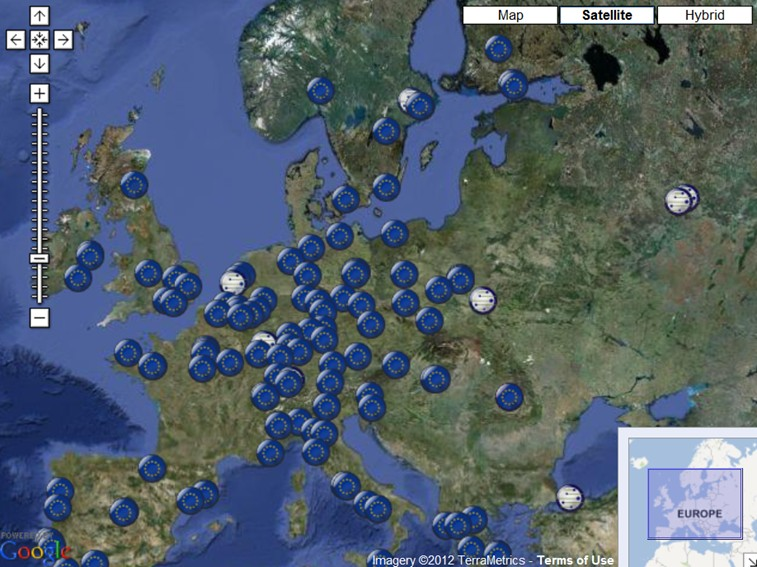
\includegraphics[width=0.6\textwidth]{statement/planetlab-europe.jpg}
\caption{Geographical distribution of PlanetLab Europe.}
\label{fig:intr-planetlab-europe}
\end{center}
\end{figure}

\subsubsection{BonFIRE}

\emph{BonFIRE} is a multi-cloud testbed based on an \ac{IaaS}
delivery model with guidelines, policies and best practices for
experimenting. Currently, \bonfire is composed by 7 geographically distributed
testbeds, which offer heterogeneous cloud services, compute resources and
storage resources.These testbeds are \emph{EPCC},\emph{ INRIA},\emph{Wellness},\emph{ HLRS}, \emph{iMinds} and \emph{PSNC}. The Figure~\ref{fig:intr-bonfire-testbeds} shows these testbeds and its interconnections.

\begin{figure}[!h]
\begin{center}
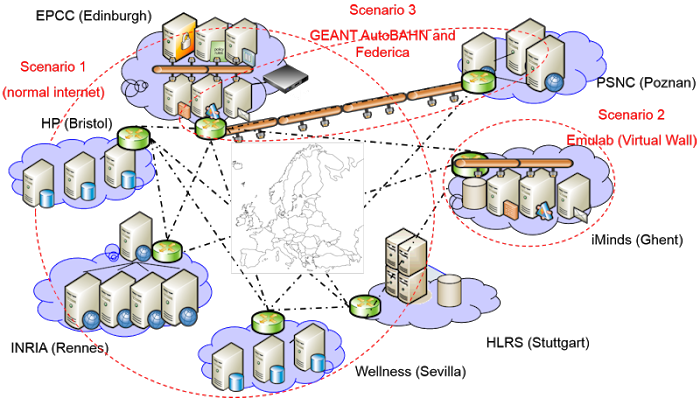
\includegraphics[width=0.7\textwidth]{statement/bonfire-testbeds.png}
\caption{BonFIRE testbeds.}
\label{fig:intr-bonfire-testbeds}
\end{center}
\end{figure}

The compute resources that \bonfire offers are summarized in Table~\ref{table:intro-instance-types}.

\begin{table}[hp]
  \centering
  {\small
  


\begin{tabular}{p{0.2\textwidth}p{0.2\textwidth}p{0.2\textwidth}p{0.2\textwidth}}
  \tabheadformat
  \tabhead{Name}   &\tabhead{CPU cores} &\tabhead{Memory} & \tabhead{Features}\\
\hline
\textit{Lite}         & 0.5 & 256 MB & \\
\hline
\textit{Small}         & 1 & 1 GB & \\
\hline
\textit{Medium}        & 2 & 2 GB & \\
\hline
\textit{Large}          & 2 & 4 GB & \\
\hline
\textit{Large+}         & 2 & 4 GB & Higher CPU clock speed\\
\hline
\textit{Large-en}        & 4 & 4 GB & \\
\hline
\textit{Xlarge}        & 4 & 8 GB & \\
\hline
\textit{Xlarge+}        & 4 & 8 GB & Higher CPU clock speed\\
\hline
\textit{Custom}        & User defined & User defined &VCPU must be an integer \\
\hline
\end{tabular}


% Local variables:
%   coding: utf-8
%   ispell-local-dictionary: "castellano8"
%   TeX-master: "main.tex"
% End:

  }
  \caption{Instance types of BonFIRE}
  \label{table:intro-instance-types}
\end{table}


The setup of compute resource can be done using contextualization variables in
order to provide important information for software applications in the virtual
machines. 
This testbed also offers elasticity resources, that are dinamically created,
updated and destroyed according to execution environment.


\subsection{Federated Tools}
\label{subsec:federatedtools}
In the breast of \emph{Fed4FIRE} project, some tools for deploying, controlling and
monitoring the experiments have been developed. 
Some of these tools are used only for developers to deploy, to provision, to
make reservations and to discover resources. These tools are \emph{Flack, Omni
  and SFI} which they have a common interface named \emph{SFA}.

The experimenters utilize the tools for controlling the experiments. These tools
are described as follows:
\begin{itemize}
\item \emph{NEPI:}The Network Experimentation Programming Interface, is a
  life-cycle management tool for network experiments. It is developed in Python
  and it provides a high-level interface to describe experiments, to provision
  resources, to control experiments and to collect all the results of the
  experiment. To highlight that this implementation provides a important way to
  manage and to make a workflow for an experiment.
\item \emph{\ac{OMF6}:} is a generic framework that allows the definition and
  orchestration of the experiments. It can be used for control the experiment
  through a distributed infrastructure based on \ac{XMPP} and an Aggregate Manager
  that manages all the information flows. It can be integrated with \ac{OML} for
  provisioning, to control and to collect all information about the experimet.
\item \emph{\ac{OML}:} this tool provides a powerful way to take input from any
  sensor or device with a software interface. This tool also defines and
  implements a reporting protocol and a collection server. On the client side,
  any application can be implemented using the \ac{OML} \ac{API} for collecting any
  information about the status of the devices concerning the experiment. 
\end{itemize}


\section{Graphical User Interfaces}

A \ac{GUI} is a software that facilitates the human-machine interaction
visually using images and graphics items. Normaly the interactions are produced
by user actions directly and these actions corresponds to events. The \ac{GUI} events
are normaly produced by the mouse, touchpad, keyboard or nowadays,a
touchscreen. When a event is located, a determinate action is performed
changing the interface itself, or creating, updating or deleting data or to
accomplish a specific proceeding. 


\subsection{Frameworks}

There are lots of graphical user interface engines or frameworks avialable for
Python. As the project is developed in Python, the user interface has to be
developed in Python also. In addition, the searched engines have to be
multiplatform. Finally, considering these above criteria, some frameworks and
libraries  as \emph{PyGUI, PyGtk, PyGame, PyQt, PyKDE and WxPython} have been studied:

\begin{itemize}
\item \emph {PyGUI:} It is a \ac{API} that provides to make graphical user interface
  easily, lightweight development and it can be used in any platform or
  operative system. The PyGUI \ac{API} offers that programmer does
  not need read any documentation because it is written in Python. It use
  PyOpenGL libraries also. It is distributed under \ac{GPL} v3.
\item \emph{PyGtk:} It is a library set of Python with which the programmer can
  develop  programs with a graphical user interface easily. It is multiplatform
  is distributed under \ac{LGPL} licence with few restrictions.
\item \emph{PyGame:} Is a set of Python modules that allows to create games and
  multimedia software as graphical user interfaces. Pygame is fully portable and
  runs on nearly every platform and operative system. This engine evolves
  funcionality of \ac{SDL} library, OpenGL and provides Blender integration. It is
  distributed under \ac{GPL} v3.
\item \emph{PyQt:} is a Python binding for Qt development. Qt is a
  cross-platform  and \ac{GUI} framework for  developing graphical user interfaces. Qt
  is distributed under \ac{GPL} v3 and \ac{LGPL} license. It is developed by Nokia and it
  permits to develop software for mobile, embedded platforms, desktop platforms
  and any operative system.
\item \emph{WxPython:} is a \ac{GUI} toolkit for Python that allows to create
  robust,highly functional graphical user interfaces esily and simply. It is
  implemented in Python and distributed under \ac{GPL} v3 license.
\end{itemize}


\section{Database}
%http://196.29.172.66:8080/jspui/bitstream/123456789/1834/1/E174.pdf
Since computer manage the users information, humans had tried to sort these data
and to collect from machines effectivelly. For this purpose, the databases were
created. The databases are conceptual models to store the information
orderly. Another step forward was the creation of the \ac{DBMS}. The \ac{DBMS}
is a software to manage the information contained into database to concentrate,
to arrange and to provide lots of mechanisms to manage the information contained
into database repository.

\subsection{DBMS}

In order to simulate the constellation of satellites for GEO-Cloud project, some
free \ac{DBMS} were studied. The most interesting for the purpose of this project are
as follows:
\begin{itemize}
%http://www.mysql.com/
\item \textbf{MySQL:}Open Source relational database management system developed by
  \emph{MySQL AB}. It is the most used database system in web applications and
  second in the world. \emph{MySQL} provides triggers, cursors, sub-selects, stored
  procedures, a embeded database library and works with distributed systems
  efficiently among others. This \ac{DBMS} is multiplatform and it works in any
  operative system. 
%https://www.monetdb.org/Home
\item \textbf{MonetDB:} Open Source column-oriented database management system
  developed by \emph{Centrum Wiskunde \& Informatica} in Netherlands. It offers
  high performance on complex queries in large databases combining tables with
  lots of columns and multi-million rows. This \ac{DBMS} is performed in data
  mining, geographic information systems and others like that.
%http://www.postgresql.org.es/
\item \textbf{PostgreSQL:} \emph{PostgreSQL} is a object-oriented relational
  distributed database management system developed by \emph{PostgreSQL Global
    Development Team}. It is distributed under \ac{BSD} license. This database use a
  client-server model based in multi-processing for garanting system stability.
\end{itemize} 

\emph{MySQL} was selected for developing because there are quite documentation and the
sintax is similar to \ac{SQL}.

\section{Distributed Systems}
%http://dl.acm.org/citation.cfm?id=1202502
%http://etheldcofie.wordpress.com/2008/08/28/distributed-computing-paradigms-traditional-client-server-or-mobile-agents/
Nowadays, almost of applications need to obtain information from other sources
or communicating with another hadware either other computers or devices. As a
result, some programming paradigms like client-server, remote procedure call and
remote object invocation were born.
\begin{itemize}
\item \textbf{Client-Server paradigm}~\\
This architecture is composed by two parts: the first one is the Server
component and the second one is the Client. The server is listening request from
Client and when a application comes, the server decodes and processed it and
sents back the reply to the Client.

\textbf{Remote Procedure Call}~\\
Remote Procedure Call uses the same principle as Client-Server but in much
complex way. Basically in remote procedure call paradigm, a client calls a
function as if it were a local function on the client machine but this called
function are located in another host that it may use to perform a function.

\textbf{Remote Object Invocation}~\\
This paradigm was born when the object-oriented programming paradigm was
developed. It is based on there are distributed objects and these objects not
necessary are fixed in a host. When a distributed-object is created, it is
binded to a set of machines as slave, so when a client application recovers that
object using a distributed-object registry or another one like that, the
provided operations by the distributed object can be remotely performed as if
it was a  operation call in applicant machine.
\end{itemize}
\subsection{Middlewares}

For client-server paradigm there are not any middleware for developing
applications. Normally this kind applications are developing using the standard
oriented socket libraries.
For \ac{RPC} development, there are several implementations as
\ac{SOAP}, \ac{CORBA}, UNIX \ac{RPC} and Pyro among others.

For Remote Object Invocation paradigm, novels middlewares are. The most used are
Hadoop and ZeroC \ac{ICE} and its features are as follows:

\subsubsection{Hadoop}
%http://hadoop.apache.org/
Hadoop is a framework for developing  reliable and scalable
distributed applications. It is based on
the architecture used by \emph{Google} named ``MapReduce'' and other componets
like \emph{Google File System}. 
Some of its componets among others are:
\begin{itemize}
\item \emph{Hadoop Common:} The common utilities for other Hadoop modules.
\item \emph{Hadoop Distributed File System:} Distributed file system that
  provides high-throughput access.
\item \emph{Hadoop YARN:}A framework for job scheduling and resource management.
\item \emph{Hadoop MapReduce:} A YARN-based system for parallel processing of
  large data sets.
\end{itemize}
It is designed for scaling up thousands of machines. It
is maintained and distributed by \emph{Apache Software Foundation} under GPL license.
 
\subsubsection{ZeroC ICE}
%http://www.zeroc.com/
\emph{ZeroC \ac{ICE}}, the internet communications engine, is a modern distributed computing
platform with support lots languages as C++,Python, Java and Ruby among others.
Permits to developers creates new powerful, efficient and simple applications
with minimal effort.
The main features of this middleware are:
\begin{itemize}
\item It is a general-purpose distributed computing platform.
\item Uses a modern and flexible specification language.
\item Dinamic invocation and dispatch.
\item Request Forwarding.
\item Asynchronous and synchronous invocation and dispatch.
\item Oneway, datagram and batched invocation.
\item Fully thread-safe.
\item Several transport protocols can be used as \ac{TCP},\ac{SSL},\ac{UDP} and also \ac{IP}v4 and
  \ac{IP}v6 are supported.
\end{itemize}

\ac{ICE} provides the following services:
\begin{itemize}
\item \emph{IceGrid:} A service for large-scale grid computing applications. 
\item \emph{IceStorm:} A sophisticated event distribution service.
\item \emph{Freeze:} Provides object persistence and the posibility to migrate
  these objects to a database.
\item \emph{Glacier2:} A firewall service.
\item \emph{IcePatch2:} A software and files distribution service.
\end{itemize} 

\section{Software Design}

In this section, the software engineering knowledges as design patters and
software portability recquired by this project was studied. These areas are
described in the following subsections.

\subsection{Multiplatform source}

One of the main objectives of GEO-Cloud consists of the software portability. As
this project is an experiment, it has to be checked in any platform with any
operative system, so the   

The developed source was written in Python. Among the huge variety of Python
interpreters, the used version for developing this project source is Python 2.7.

\emph{GNU/Linux} was the platform in which the development of all project files were
carried out. Besides the libraries distributed within Python, \emph{Paramiko}
Python library was used. This library implements \ac{SSH} protocol operations
for managing and controlling machines remotely. This library is distributed
under \ac{GPL} v3.
http://www.lag.net/paramiko/  

\subsection{Software Development Life Cycles}

Several methodologies for software development are. Historically, the software
was developed without any methodology, so there were lots of bugs in the
code. As a result, programs did not work correctly or they were inefficient or
inclusive, they stoped unexpectedly. Then the savior programmer tried to solve
the trouble wasting lot of time. Thus, the software development is very
expensive. 
At present, the software development is guided by life cycles. In this cycles,
stages as planning, designing, implementation, testing, documenting, deployment
and maintenance are basics for software development. Depending on how these
stages are done, several life cicles are. Among others, the most important and
more used are:
\begin{itemize}
\item \emph{Waterfall model:} strict model in which developers have to follow these
  stages in order: analisys,design, implementation, testing, deployment and maintenance.
\item \emph{Spiral model:} this life cicle combines the waterfall model and rapid
  prototyping.
\item \emph{Iterative and incremental cicle:} it bases on the development of small but
  ever-larger portions of a software. During software development, several
  iterations may be in progress at the same time. Using this cycle, the
  end-users can check the no-ended product for updating requirements or to give feedback
  to end-user.
\item \emph{Agile development:} This model is very used nowadays, and its principles
  are the iterative development, to incorporate continuous feedback and
  stages iterations. 
\end{itemize}

\subsection{Design Patterns}

The software programming patterns that were studied for developing GEO-Cloud
are:
\begin{itemize}
\item Singleton: only a single instance of a class can exist.
\item Composite: a tree structure of simple and composite objects.
\item Proxy: an object that represents another one.
\end{itemize}

\subsection{Testing}

At the same time the development of GEO-Cloud software, the testing process was
done also. The testing was made by two ways: hand testing and test-case oriented
testing. In case of the second one, sundry testing frameworks were studied.
The selected framework for testing in Python was \emph{UnitTest} and its
extension \emph{Nose}. It is included in Python standard library, is easy to use
and it has lots of plugins. 

The developed test-cases were black-box essentialy. Some white box test-cases
were developed but the code coverage was not thorough. 
